\documentclass[11pt, aspectratio=169]{beamer}
% Theme adapted from the unofficial SMU Beamer template by Felix Nie (CC BY 4.0), https://github.com/felixnie/smu-beamer
% Colours and layout kept; the SMU logo and campus background are replaced by the Strathmore University logo.

\usepackage{booktabs}
\usepackage{array}
\newcolumntype{L}[1]{>{\raggedright\arraybackslash}p{#1}}
\setlength{\abovedisplayskip}{1pt}\setlength{\belowdisplayskip}{1pt}\setlength{\abovedisplayshortskip}{0pt}\setlength{\belowdisplayshortskip}{0pt}
\newcommand{\body}{\fontsize{6.6}{7.9}\selectfont}
\newcommand{\bodys}{\fontsize{6.0}{7.2}\selectfont}
\newcommand{\chip}[2]{\colorbox{#1}{\parbox{\dimexpr\linewidth-2\fboxsep\relax}{\textcolor{white}{\textbf{\scriptsize #2}}}}}
\hyphenpenalty=10000 \exhyphenpenalty=10000 \tolerance=2000 \emergencystretch=2em

\usepackage{tikz}
\usetikzlibrary{arrows.meta,positioning,shapes.geometric}
\setbeamerfont{footnote}{size=\tiny}
\newcommand{\citep}[1]{(#1)}
\usetheme{Madrid}
\definecolor{navy}{RGB}{21, 28, 85}
\definecolor{gold}{RGB}{198, 146, 0}
\setbeamercolor*{structure}{bg=navy, fg=navy}
\setbeamercolor*{palette primary}{use=structure, fg=white, bg=navy}
\setbeamercolor*{palette secondary}{use=structure, fg=navy, bg=white}
\setbeamercolor*{palette tertiary}{use=structure, fg=white, bg=navy}
\setbeamercolor{frametitle}{bg=navy, fg=white}
\setbeamercolor*{titlelike}{parent=palette primary}
\setbeamercolor{section in head/foot}{fg=white, bg=gold}
\setbeamercolor{headline}{fg=white, bg=gold}
\setbeamercolor{item projected}{bg=gold}
\setbeamertemplate{enumerate items}{bg=gold}
\setbeamercolor{itemize item}{fg=gold}
\setbeamercolor{itemize subitem}{fg=gold}
\setbeamercolor{button}{bg=gold}
\setbeamercolor{section in toc}{fg=black}
\setbeamercolor{block title}{bg=gold, fg=white}
\setbeamercolor{block body}{bg=gold!20}
\setbeamercolor{block title alerted}{bg=orange, fg=white}
\setbeamercolor{block body alerted}{bg=orange!10}
\setbeamercolor{block title example}{bg=navy, fg=white}
\setbeamercolor{block body example}{bg=navy!10}

\usefonttheme{default}
\usepackage{palatino}
\usepackage[default]{opensans}
\useinnertheme{circles}
\useoutertheme{miniframes}
\setbeamertemplate{headline}{
  \nointerlineskip
  \begin{beamercolorbox}[wd=\paperwidth,ht=7.0ex]{headline}
    \insertnavigation{\paperwidth}\vspace*{2.0ex}
  \end{beamercolorbox}}
\setbeamertemplate{navigation symbols}{}
\setbeamerfont{institute}{size=\scriptsize}
\setbeamerfont{date}{size=\footnotesize}
\setbeamerfont{author}{size=\footnotesize}
\setbeamersize{text margin left=1cm, text margin right=1.5cm}


\newcommand{\compact}{\fontsize{9.4}{11.2}\selectfont}
\newcommand{\bridge}[1]{\vfill\par{\footnotesize\itshape\color{navy}$\rightarrow$\ #1}}


\graphicspath{{../results/}}

\title[Federated Potato Disease Detection]{Federated Deep Learning for Privacy-Preserving Potato Disease Detection: a Pipeline and Model Service}
\author[G.\ C.\ Ngetich, 221855]{Gracious Chepkemoi Ngetich\\ \smallskip DSA 8401 Applied Machine Learning, Capstone}
\institute[Strathmore University]{Master of Science in Data Science and Analytics\\ \smallskip Strathmore University, iLabAfrica}
\date[November 2026]{24 November 2026}

\hypersetup{colorlinks=true, citecolor=gold, linkcolor=navy, urlcolor=navy}
\begin{document}

\logo{
\includegraphics[height=1.0cm]{logo.jpg}}
\section{}
\begin{frame}
  \titlepage
\end{frame}
\setbeamercolor{section in head/foot}{fg=gold, bg=white}
\setbeamercolor{title in head/foot}{fg=white, bg=gold}
\setbeamercolor{headline}{fg=gold, bg=white}

% ------------------------------------------------------------------ problem
\section{Problem}
\begin{frame}[t]{The Problem: Early Disease Screening Without Pooling Photos}
  \body
  \begin{columns}[T]
    \begin{column}{0.485\textwidth}
      \chip{navy}{Why it matters in Kenya}\par\vspace{0.25em}
      \begin{itemize}\setlength\itemsep{0.2em}
        \item About 800,000 smallholders grow potato, the second food crop after maize (CIP 2021; MoALFC 2021).
        \item Bacterial wilt was on over 70\% of surveyed farms in 2014 and spreads through infected seed tubers (Muthoni et al.\ 2014).
        \item Only 4.9\% of surveyed farmers used certified seed (Kwambai et al.\ 2024).
        \item Laboratory tests destroy the sample and need equipment farmers lack, so a cheap photo screen is useful, if it says how sure it is.
      \end{itemize}
    \end{column}
    \begin{column}{0.485\textwidth}
      \chip{gold}{What this project builds}\par\vspace{0.25em}
      \begin{itemize}\setlength\itemsep{0.2em}
        \item A system that classifies a potato \textbf{leaf or tuber photo into 16 classes} (7 leaf, 9 tuber, healthy included) and serves the answer through an API.
        \item Trained with \textbf{federated learning}: each simulated farm keeps its photos and sends only model updates (McMahan et al.\ 2017).
        \item Farms differ in disease mix, which breaks the identical-data assumption of federated averaging (Hsu et al.\ 2019; Li et al.\ 2020).
      \end{itemize}\par\vspace{0.4em}
      \begin{block}{Question}
        How much accuracy does federation cost against central training, and which settings recover it?
      \end{block}
    \end{column}
  \end{columns}
\end{frame}

% -------------------------------------------------------------- architecture
\section{System}
\begin{frame}[t]{The System End to End}
  \body
  \centering
  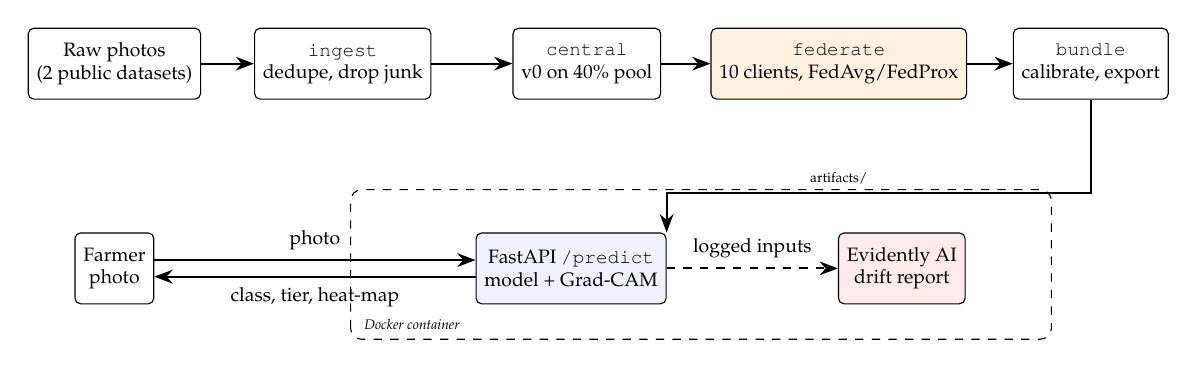
\begin{tikzpicture}[font=\scriptsize, box/.style={draw, rounded corners=2pt, align=center, inner sep=3pt, fill=white, minimum height=0.9cm}, arr/.style={-{Stealth}, thick}]
    \node[box] (raw) at (0.2,0) {Raw photos\\(2 public datasets)};
    \node[box] (cl) at (3.1,0) {\texttt{ingest}\\dedupe, drop junk};
    \node[box] (v0) at (6.2,0) {\texttt{central}\\v0 on 40\% pool};
    \node[box, fill=orange!12] (fl) at (9.4,0) {\texttt{federate}\\10 clients, FedAvg/FedProx};
    \node[box] (bd) at (12.6,0) {\texttt{bundle}\\calibrate, export};
    \draw[arr] (raw)--(cl); \draw[arr] (cl)--(v0); \draw[arr] (v0)--(fl); \draw[arr] (fl)--(bd);
    \node[box] (ph) at (0.2,-2.6) {Farmer\\photo};
    \node[box, fill=blue!6] (api) at (6.0,-2.6) {FastAPI \texttt{/predict}\\model + Grad-CAM};
    \node[box, fill=red!8] (mon) at (10.2,-2.6) {Evidently AI\\drift report};
    \draw[arr] (bd.south) |- ([yshift=0.5cm]api.north east) -- (api.north east);
    \node[font=\tiny] at (9.4,-1.45) {artifacts/};
    \draw[arr] ([yshift=3pt]ph.east)--node[above]{photo}([yshift=3pt]api.west);
    \draw[arr] ([yshift=-3pt]api.west)--node[below]{class, tier, heat-map}([yshift=-3pt]ph.east);
    \draw[arr, dashed] (api)--node[above]{logged inputs}(mon);
    \draw[dashed, rounded corners] (3.2,-3.5) rectangle (12.1,-1.6);
    \node[font=\tiny\itshape, anchor=south west] at (3.25,-3.5) {Docker container};
  \end{tikzpicture}\par\vspace{0.6em}
  \begin{tabular}{@{}L{0.30\textwidth}L{0.30\textwidth}L{0.30\textwidth}@{}}
    \textbf{Scripted pipeline} \par every stage runs from the command line, resumable, no notebook. &
    \textbf{Model service} \par FastAPI in Docker: class, calibrated confidence, tier, heat-map. &
    \textbf{Monitoring} \par the service never sees labels, so it watches the photos for drift.
  \end{tabular}
\end{frame}

% --------------------------------------------------------------------- data
\section{Data}
\begin{frame}[t]{Data: Raw Photos, Cleaned, and One Deliberate Complication}
  \body
  \begin{columns}[T]
    \begin{column}{0.52\textwidth}
      \chip{navy}{Cleaning (scripted, every removal logged)}\par\vspace{0.25em}
      \bodys
      \begin{tabular}{@{}lrr@{}}\toprule & Leaf & Tuber \\\midrule
        Raw photos & 3,076 & 3,905 \\
        Catch-all class dropped & 0 & 74 \\
        Identical, conflicting labels & 12 & 26 \\
        Identical copies & 49 & 0 \\
        Near-identical (64-bit hash) & 36 & 11 \\\midrule
        \textbf{Kept} & \textbf{2,979} & \textbf{3,794} \\
        Imbalance, largest : smallest & 10.9 : 1 & 30.0 : 1 \\\bottomrule
      \end{tabular}\par\vspace{0.5em}
      \body
      Duplicates across the train and test split inflate scores, and a copy filed under two diseases is a wrong label for one of them.
    \end{column}
    \begin{column}{0.455\textwidth}
      \chip{gold}{Splits, imbalance and simulated farms}\par\vspace{0.25em}
      \begin{itemize}\setlength\itemsep{0.2em}
        \item Stratified 70/15/15 split once per seed. The test set (1,016 photos) is never used for tuning.
        \item Imbalance kept, handled by a capped class-weighted loss and macro-F1.
        \item Neither dataset is Kenyan, so clients are simulated: a \textbf{Dirichlet label split} over 10 clients. $\alpha=100$ means near-identical farms, $\alpha=0.1$ gives each farm a few dominant classes (Hsu et al.\ 2019).
        \item 40\% of training photos form a central pool for the starting model v0. The other 60\% belong to the farms.
      \end{itemize}
    \end{column}
  \end{columns}
\end{frame}

% --------------------------------------------------------------- techniques
\section{Methods}
\begin{frame}[t]{Techniques Chosen, and Techniques Left Out}
  \body
  \begin{columns}[T]
    \begin{column}{0.485\textwidth}
      \chip{navy}{Chosen, and why}\par\vspace{0.25em}
      \begin{itemize}\setlength\itemsep{0.2em}
        \item \textbf{MobileNetV2, ImageNet-pretrained} (2.3 M parameters): small enough for phones and for repeated federated rounds on a CPU.
        \item \textbf{Central stage, then FedAvg and FedProx} on the whole network, one local epoch, 30 rounds, local learning rate $10^{-5}$ picked on validation.
        \item \textbf{Temperature scaling} so the confidence is a probability (Guo et al.\ 2017), reported as three tiers.
        \item \textbf{Grad-CAM} for where the model looked (Selvaraju et al.\ 2017). With pooling plus a linear head it is exact in closed form: one forward pass, no gradients.
        \item \textbf{Evidently AI} drift tests on brightness, contrast, sharpness, colour and size of incoming photos.
      \end{itemize}
    \end{column}
    \begin{column}{0.485\textwidth}
      \chip{gold}{Ruled out, and why}\par\vspace{0.25em}
      \begin{itemize}\setlength\itemsep{0.2em}
        \item \textbf{Vision Transformers, large CNNs}: too heavy for phones on slow links.
        \item \textbf{LLM, RAG, agents}: nothing to do in image classification.
        \item \textbf{SHAP}: Grad-CAM answers ``where in the photo'' directly; pixel SHAP costs hundreds of passes per request.
        \item \textbf{Boosting on hand-made features}: pretrained convolutional features capture leaf and tuber texture far better.
        \item \textbf{DP-SGD, secure aggregation}: they address a different threat, and with 10 clients the budget would be too weak to claim anything. No formal privacy guarantee is claimed.
        \item \textbf{SCAFFOLD, FedAdam}: FedAvg and FedProx already give the baseline and the standard heterogeneity fix.
      \end{itemize}
    \end{column}
  \end{columns}
\end{frame}

% ------------------------------------------------------------------ results
\section{Results}
\begin{frame}[t]{Results 1: Label Skew and Algorithm}
  \body
  \begin{columns}[T]
    \begin{column}{0.47\textwidth}
      \centering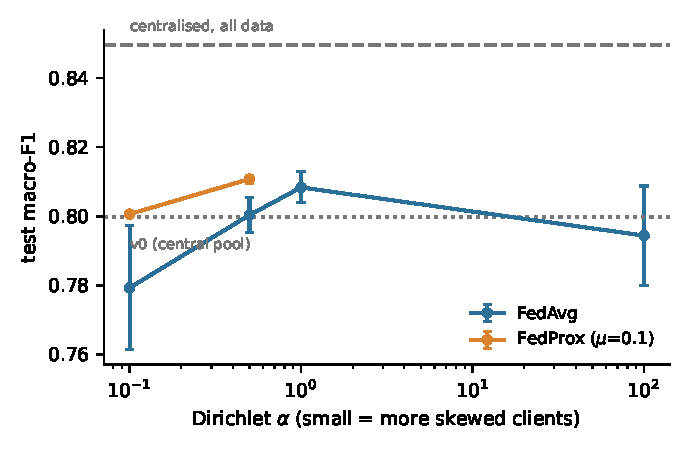
\includegraphics[height=4.0cm]{fig_alpha.pdf}\par
      {\tiny Test macro-F1 against Dirichlet $\alpha$ (small = more skewed).}
    \end{column}
    \begin{column}{0.51\textwidth}
      \chip{navy}{Test macro-F1}\par\vspace{0.25em}
      \bodys\centering\begin{tabular}{rrcc}
\toprule
$\alpha$ & label skew (JS) & FedAvg macro-F1 & FedProx macro-F1 \\
\midrule
100 & 0.00 & 0.794 $\pm$ 0.014 (n=2) & -- \\
1 & 0.11 & 0.808 $\pm$ 0.004 (n=2) & -- \\
0.5 & 0.13 & 0.800 $\pm$ 0.005 (n=2) & 0.811 $\pm$ 0.001 (n=2) \\
0.1 & 0.32 & 0.779 $\pm$ 0.018 (n=2) & 0.801 (n=1) \\
\midrule
\multicolumn{2}{l}{v0 (central pool only)} & \multicolumn{2}{c}{0.800 $\pm$ 0.010 (n=3)} \\
\multicolumn{2}{l}{Centralised, all data} & \multicolumn{2}{c}{0.850 $\pm$ 0.007 (n=3)} \\
\bottomrule
\end{tabular}\par\vspace{0.3em}
      \body\raggedright
      \begin{itemize}\setlength\itemsep{0.15em}
        \item \textbf{FedAvg averages about 0.80}: the same as v0, five points under centralised training (0.850). It gained 1.7 points over v0 on seed 42 and lost 0.3 on seed 43.
        \item \textbf{FedProx at $\alpha=0.5$ reaches 0.811}, above FedAvg and above v0 on both seeds. Two seeds: a consistent sign, not a firm ranking.
        \item Skew has a mild effect: only $\alpha=0.1$ stands out, and only just.
      \end{itemize}
    \end{column}
  \end{columns}
\end{frame}

\begin{frame}[t]{Results 2: The Cheapest Update Is as Good as the Whole Network}
  \body
  \chip{navy}{What a client trains and sends each round ($\alpha=0.5$), test macro-F1}\par\vspace{0.3em}
  \centering\resizebox{0.92\linewidth}{!}{\begin{tabular}{lrrc}
\toprule
Setting ($\alpha=0.5$) & parameters sent & MB per client per round & macro-F1 \\
\midrule
Full network from v0 (default) & 2,210,256 & 8.84 & 0.800 $\pm$ 0.005 (n=2) \\
Last blocks from v0 & 430,096 & 1.72 & 0.803 $\pm$ 0.003 (n=2) \\
Classifier head only from v0 & 20,496 & 0.08 & 0.796 $\pm$ 0.003 (n=2) \\
Full network, no central stage (empty head) & 2,210,256 & 8.84 & 0.287 $\pm$ 0.000 (n=2) \\
\bottomrule
\end{tabular}}\par\vspace{0.4em}
  \begin{columns}[T]
    \begin{column}{0.60\textwidth}
      \raggedright
      \begin{itemize}\setlength\itemsep{0.15em}
        \item Classifier head only: \textbf{80 KB per round} against 8.84 MB, a difference of at most 0.007 in macro-F1, about the seed spread.
        \item Over 30 rounds a client uploads about 2.4 MB instead of 265 MB.
        \item \textbf{The central stage is not optional}: from the ImageNet backbone with an empty head the full network reaches only 0.287 after 30 rounds, on both seeds.
      \end{itemize}
    \end{column}
    \begin{column}{0.36\textwidth}
      \centering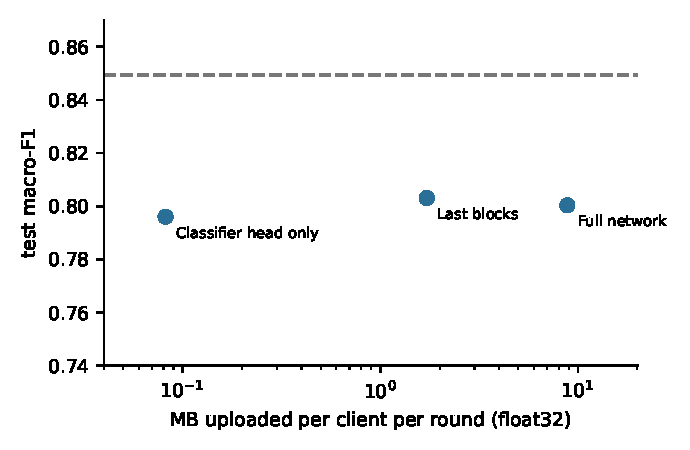
\includegraphics[height=2.9cm]{fig_scope.pdf}
    \end{column}
  \end{columns}
\end{frame}

\begin{frame}[t]{Results 3: The Shipped Model, Its Confidence and Its Weak Spots}
  \body
  \begin{columns}[T]
    \begin{column}{0.40\textwidth}
      \chip{gold}{Calibrated tiers (test set)}\par\vspace{0.25em}
      \bodys
      \begin{tabular}{@{}lrr@{}}\toprule Tier & share & accuracy \\\midrule
        very likely & 66.6\% & 97.6\% \\
possible & 27.9\% & 67.8\% \\
unsure & 5.5\% & 33.9\% \\\bottomrule
      \end{tabular}\par\vspace{0.4em}
      \body
      Temperature scaling ($T=1.22$) cuts the expected calibration error from 0.050 to 0.029. A ``very likely'' answer can be trusted far more than an ``unsure'' one.
    \end{column}
    \begin{column}{0.56\textwidth}
      \chip{navy}{Shipped model (FedAvg, $\alpha=0.5$, seed 42): 0.805}\par\vspace{0.25em}
      \begin{itemize}\setlength\itemsep{0.2em}
        \item Reliable tuber classes: F1 at or above 0.93 for Blackspot Bruising, Brown Rot, Dry Rot, Healthy, Soft Rot.
        \item Weak: leaf Fungi, Pest and Phytophthora (F1 0.62 to 0.67). Pest is read as Fungi in 25 of 89 photos.
        \item Rare tuber classes (Blackleg, Common Scab: 7 test photos each) score about 0.55 to 0.59 and are noisy.
        \item On 16 held-out sample photos through the live service: 12 right, 11 ``very likely'' and correct, and all 4 misses only ``possible''. This is what the tiers are for.
      \end{itemize}
    \end{column}
  \end{columns}
\end{frame}

% ------------------------------------------------------------------ service
\section{Deployment}
\begin{frame}[t]{The Model Service: Answer, Confidence, Heat-map}
  \body
  \begin{columns}[T]
    \begin{column}{0.30\textwidth}
      \centering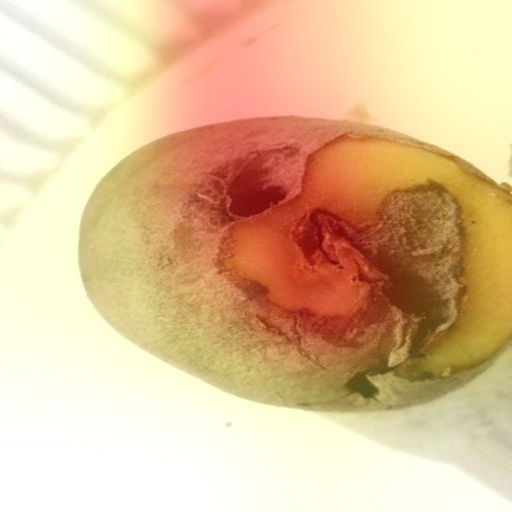
\includegraphics[height=3.6cm]{fig_cam.png}\par
      {\tiny Held-out dry-rot tuber, predicted Dry Rot at 99\%: the highlight sits on the lesion.}
    \end{column}
    \begin{column}{0.66\textwidth}
      \chip{navy}{\texttt{docker compose up}, then send a photo}\par\vspace{0.25em}
      \bodys
      \begin{tabular}{@{}L{0.30\linewidth}L{0.64\linewidth}@{}}\toprule
        \texttt{POST /predict} & top 3 classes, calibrated probabilities, tier, advice, optional heat-map PNG \\
        \texttt{GET /model} & version, temperature, test metrics \\
        \texttt{GET /healthz} & liveness, used by the container health check \\
        \texttt{GET /drift} & Evidently drift summary of the last 500 requests against the training photos: K-S per column, drift if any column's $p<0.05/7$ \\
        \texttt{GET /} & upload page that works on a phone browser \\\bottomrule
      \end{tabular}\par\vspace{0.4em}
      \body
      Bad input is refused: 422 for non-images and photos under 64 px, 413 above 10 MB. Checked on the running container: ordinary photos give no drift; dark, oversized and blurry photos are each flagged.
    \end{column}
  \end{columns}
\end{frame}

\begin{frame}[t]{Reproducible by a Reviewer in Minutes, Not Days}
  \body
  \renewcommand{\arraystretch}{1.1}
  \begin{tabular}{@{}cL{0.27\textwidth}rL{0.45\textwidth}@{}}
    \toprule
    \textbf{Level} & \textbf{Command} & \textbf{Time} & \textbf{What it shows} \\
    \midrule
    0 & \texttt{docker compose up}\par\texttt{make test} & about 10 min & Deployed service works; 21 tests pass \\
    1 & \texttt{make smoke} & about 10 min & Every stage runs end to end on a 192-photo mini dataset, no download \\
    2 & \texttt{make review} & about 25 min & Real data, 10 real federated rounds from the shipped v0, calibration \\
    3 & \texttt{make full} & about 7 h per seed & The whole experiment grid; resumable \\
    \bottomrule
  \end{tabular}\par\vspace{0.6em}
  \begin{itemize}\setlength\itemsep{0.2em}
    \item The recorded runs of the grid ship in \texttt{results/}, and every table and figure in the report and in these slides is rebuilt from them.
    \item CI runs the tests and the smoke run on every push. \texttt{AI\_USE.md} discloses the AI assistance.
  \end{itemize}
\end{frame}

% ------------------------------------------------------------- limits + end
\section{Conclusion}
\begin{frame}[t]{Limitations}
  \body
  \begin{columns}[T]
    \begin{column}{0.485\textwidth}
      \begin{itemize}\setlength\itemsep{0.25em}
        \item Clients are simulated from two public, non-Kenyan datasets. The skew parameter varies disease mix only, not camera, light, season or place.
        \item Test photos come from the same sources as training photos. Field accuracy will be lower, and the drift monitor can say inputs moved, not that accuracy fell.
        \item Leaf photos are 1,500 px and tuber photos 224 px, so organ is partly recognisable from image statistics: the 16-class score is easier than a single-organ score.
      \end{itemize}
    \end{column}
    \begin{column}{0.485\textwidth}
      \begin{itemize}\setlength\itemsep{0.25em}
        \item Two seeds (42 and 43); FedProx at $\alpha=0.1$ has one. Differences under about one point cannot be told apart.
        \item Several classes have 7 test photos, so their F1 is noisy.
        \item Federation keeps photos on the client. It gives no formal privacy guarantee on the updates, and none is claimed.
        \item The service is a screening aid, not a diagnosis, and its advice text says so.
      \end{itemize}
    \end{column}
  \end{columns}
\end{frame}

\begin{frame}[t]{Conclusion}
  \body
  \begin{columns}[T]
    \begin{column}{0.485\textwidth}
      \chip{navy}{Delivered}\par\vspace{0.25em}
      \begin{itemize}\setlength\itemsep{0.25em}
        \item A scripted, resumable pipeline from raw photos to a calibrated model.
        \item A Dockerised FastAPI service with calibrated tiers, Grad-CAM and drift monitoring.
        \item 21 tests, CI, a mini-dataset smoke run, and a documented reviewer path.
        \item A report with every number traceable to the shipped run records.
      \end{itemize}
    \end{column}
    \begin{column}{0.485\textwidth}
      \chip{gold}{Found}\par\vspace{0.25em}
      \begin{itemize}\setlength\itemsep{0.25em}
        \item Centralised training (0.850) beats federated (FedAvg about 0.80, FedProx 0.811): federation recovered at most one to two points of the five-point gap over the central starting model.
        \item The starting point matters more than label skew: no central stage gives 0.287.
        \item Updating only the classifier head (80 KB) matches the whole network (8.84 MB), so communication cost is not paid for in accuracy.
      \end{itemize}
    \end{column}
  \end{columns}
  \bridge{Code, report and artifacts are in one repository; \texttt{README.md} gives the commands for each level.}
\end{frame}

\section{References}
\begin{frame}[t]{References}
  \bodys
  \setlength\parskip{0.25em}
  CIP (2021). \emph{Feed the Future USAID Kenya Accelerated Value Chain Development Program. Potato Value Chain. Six-Year Final Report}. International Potato Center.\par
  Guo, C., Pleiss, G., Sun, Y., Weinberger, K. Q. (2017). On calibration of modern neural networks. \emph{ICML}.\par
  Hsu, T.-M. H., Qi, H., Brown, M. (2019). Measuring the effects of non-identical data distribution for federated visual classification. \emph{arXiv:1909.06335}.\par
  Islam, S., Afrin, T. (2025). PotatoCare: deep learning based potato disease dataset, v2. \emph{Mendeley Data}, doi:10.17632/7vm7xskfg4.2.\par
  Kwambai, T. K. et al.\ (2024). Seed quality and variety preferences amongst potato farmers in North-Western Kenya: lessons for the adoption of new varieties. \emph{Potato Research}, 67(1).\par
  Li, T., Sahu, A. K., Zaheer, M., Sanjabi, M., Talwalkar, A., Smith, V. (2020). Federated optimization in heterogeneous networks. \emph{MLSys}.\par
  McMahan, B., Moore, E., Ramage, D., Hampson, S., Aguera y Arcas, B. (2017). Communication-efficient learning of deep networks from decentralized data. \emph{AISTATS}.\par
  Muthoni, J., Kabira, J. N., Shimelis, H., Melis, R. (2014). Spread of bacterial wilt disease of potatoes in Kenya: who is to blame? \emph{International Journal of Horticulture}, 4(3).\par
  MoALFC (2021). \emph{The National Potato Strategy 2021-2025}. Government of Kenya.\par
  Sandler, M., Howard, A., Zhu, M., Zhmoginov, A., Chen, L.-C. (2018). MobileNetV2: inverted residuals and linear bottlenecks. \emph{CVPR}.\par
  Selvaraju, R. R. et al.\ (2017). Grad-CAM: visual explanations from deep networks via gradient-based localization. \emph{ICCV}.\par
  Shabrina, N. H. et al.\ (2023). Potato leaf disease dataset in uncontrolled environment. \emph{Mendeley Data}.
\end{frame}

\end{document}
